\section{Results}
\label{results}

We present empirical findings from both simulation and test network (Amity) data
to verify the behaviour of the algorithm. The next few sections are laid out as
follows: we pick a property of the protocol that we're interested in verify and
present simulation results to depict the behaviour. Following that we present 
(if applicable) results from the test net depicting the same behaviour.

\subsection{Setup}

The simulation is set up as a game between two actors: the honest network, and
the attacker (in some setups). The game starts at a point in time given some initial state,
$I=(td_w,td_s,d_w,d_s)$. Where $td_w, td_s$ refers to the total staking or
working difficulty at block $n-1$, and $d_w, d_s$ refers to the last difficulty
or the PoW and PoS blocks.

For the purposes of some experiments, we generate the block generation scheme
for the honest party and observe results. For others, we simulate both parties. This
is done by allotting both parties with a time interval, and running a running a
random walk following the rules of the protocol. In scenarios where we want to
observe attacker success rate (for example, in the case of the double spend), we
repeatedly run a random walk to observe success rates at various power ratios.

\subsection{Block Generation Fairness}

We start with examining block generation fairness, by examining a few scenarios,
we examine through simulation the base case of two players, one with static
hash rate and voting power, another that we will vary and examine. For these
simulation we always assume the network is in a \textbf{steady state}. We define
a steady state as the following, given $H$ is the network total hashing power,
and $V$ is the network total voting power. Then steady state is when these two
variables are constant, and $d_s = V \cdot T$, $d_w = H \cdot T$.

\begin{figure}[h]
    \centering
    \begin{tabular}{| c || c |}
        \hline
        \multicolumn{2}{| c |}{\textbf{Equal Power Scenario}} \\
        \hline
        Total Blocks Generated &  252575 \\
        Block Generation Ratio (Total) & 0.5000 \\
        Block Generation Ratio (PoS) & 0.5002 \\
        Block Generation Ratio (PoW) & 0.4997 \\
        \hline
        \multicolumn{2}{| c |}{\textbf{2x Hash Rate, No Voting Power Scenario}} \\
        \hline
        Total Blocks Generated & 252619 \\
        Block Generation Ratio (Total) & 0.3331\\
        Block Generation Ratio (PoS) & 0 \\
        Block Generation Ratio (PoW) & 0.6662 \\
        \hline
        \multicolumn{2}{| c |}{\textbf{2x Voting Power, No Voting Power Scenario}} \\
        \hline
        Total Blocks Generated & 253135 \\
        Block Generation Ratio (Total) & 0.3327 \\
        Block Generation Ratio (PoS) & 0.6654 \\
        Block Generation Ratio (PoW) & 0 \\
        \hline
    \end{tabular}
    \caption{Attacker block production under various scenarios. This data was
    generated at steady state conditions, with a time allotment of 30 days.}
    \label{tab:table_block_fairness}
\end{figure}

We examine the block production with a time allotment of 30 days, the results are
depicted in figure \ref{tab:table_block_fairness}. We examine two cases here: First, when
the examined player has equal hashing and voting power (same resource) with the other. In this case the
expected rewards for both players should be identical. We see this is true in the \textbf{Equal
Power Scenario} as block production for both sides are identical.

Second, we examine a scenario where the examined player has majority dominance in one resource,
expectation is that one resource can at most only obtain 50\% of the rewards due to the interleaving
structure of the blockchain. The percentage of blocks mined (at steady state) should
on average be,

\begin{equation}
    P(win) = \frac{1}{2}v_i/\sum_i{v_i} + \frac{1}{2}h_i/\sum_i{h_i}
\end{equation}

in examples two and three, in which the examined player had twice the hash rate and voting power.
In both cases, they produced blocks as expected according to our probability equation.

\subsection{Block Time Distribution}

Then, we look at the block time distribution based on our simulation. As described earlier, the protocol
difficulty adjustment function targets a mean block time of $T$ seconds, which is set in the simulations
and on Amity to be 10 seconds. The distribution of PoS/PoW/All block deltas fits well the exponential distribution, as shown in
figure \ref{fig:pos_pow_delta_histogram}.

\begin{figure}[h]
    \centering
    \begin{tabular}{| c || c | c |}
        \hline
        \multicolumn{3}{| c |}{\textbf{$E$ and $\sigma$ of Simulations and Amity}} \\
        \hline
        & Mean & Standard Deviation \\
        \hline
        Simulations PoW & 10.1965 & 10.6469 \\
        Simulations PoS & 10.1174 & 10.3223 \\
        Amity PoW & 9.6748 & 11.5929 \\
        Amity PoS & 9.8408 & 10.2822 \\
        \hline
    \end{tabular}
    \caption{Caption}
    \label{fig:block_time_mean_std}
\end{figure}

\begin{figure}[h]
    \centering
    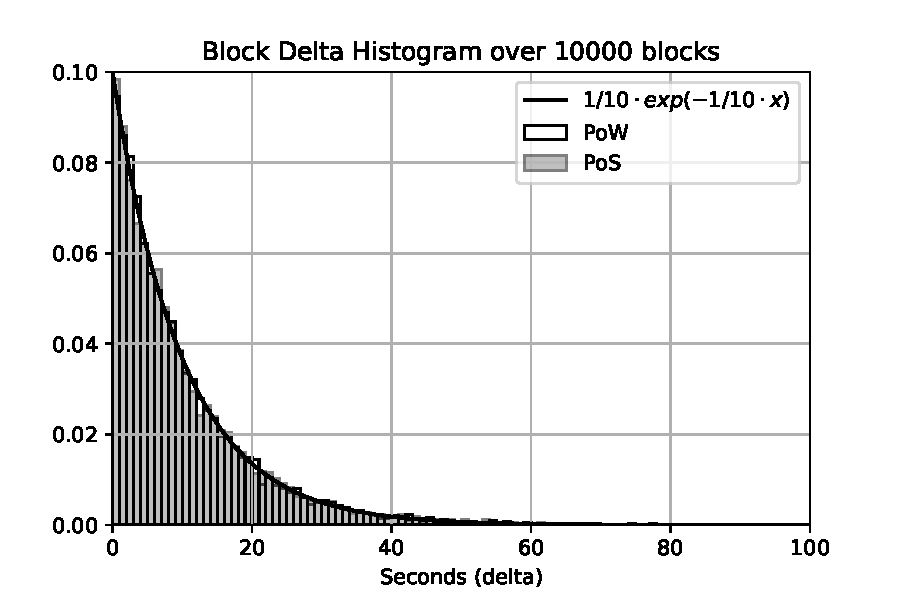
\includegraphics[width=0.55\linewidth]{assets/sim_results/block_delta_histogram_steady_state.pdf}
    \caption{Histogram of PoW and PoS block generation at
    steady state (without perturbation of hashing or voting power). This plot was
    generated using 100 bins with 1 second spacing. We conclude that at steady
    state, the two generation algorithms exhibit extremely similar exponential
    PDFs, with $\lambda = \frac{1}{10}$ (rate).}
    \label{fig:pos_pow_delta_histogram}
\end{figure}

\begin{figure}[h]
    \centering
    \subfloat[PoW]{{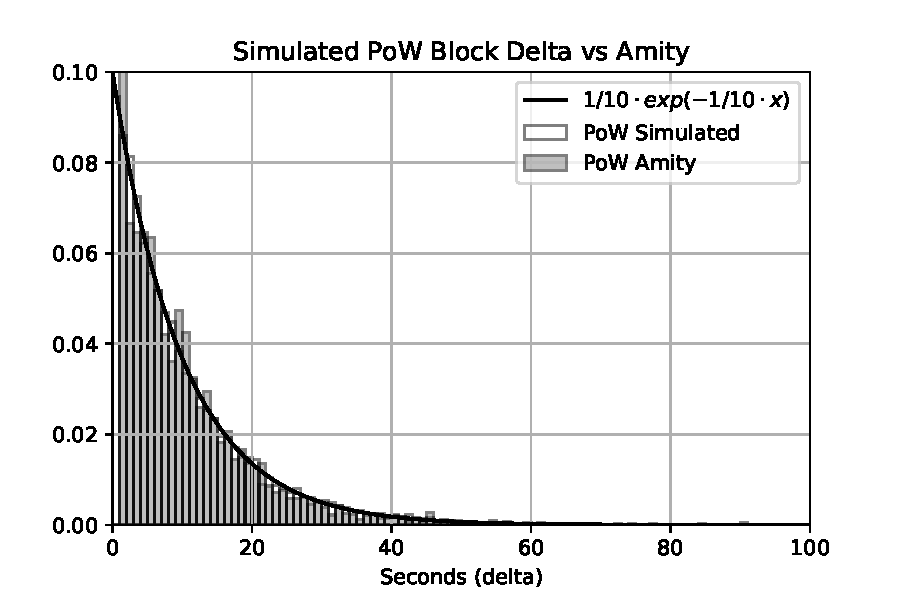
\includegraphics[width=0.45\linewidth]{assets/sim_results/pow_block_delta_histogram.pdf} }}
    \qquad
    \subfloat[PoS]{{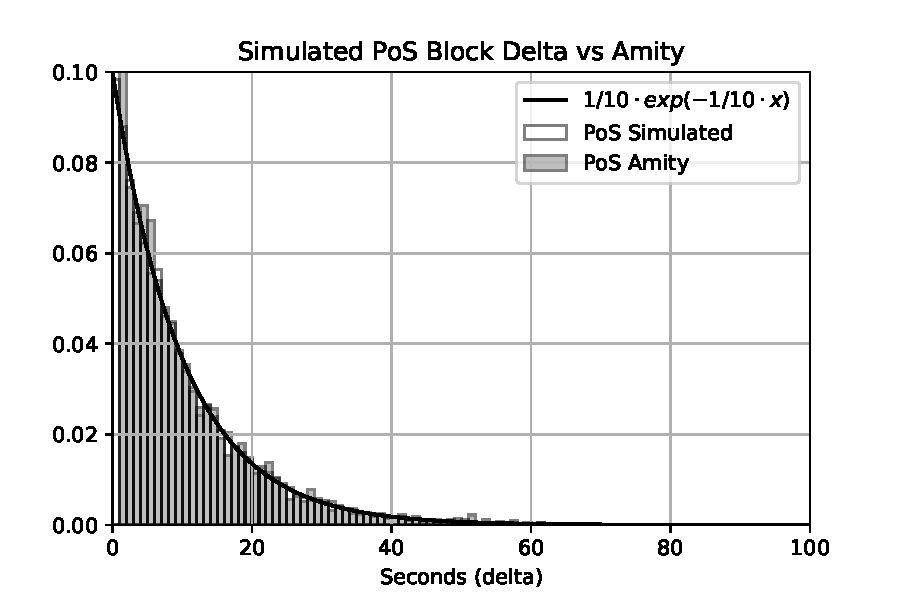
\includegraphics[width=0.45\linewidth]{assets/sim_results/pos_block_delta_histogram.pdf} }}
    \caption{Density histogram of simulated block deltas, vs. data from Amity. Data was retrieved from a set of 10000 consecutive blocks, starting from block 300.}
    \label{fig:delta_histogram}
\end{figure}

We also verify that similar behaviour is shown on the live Amity network, these results show us
that the simulation results are somewhat representative of reality as seen by their similarities
in figure \ref{fig:delta_histogram}. We attribute
the differences in results to the effects of network delay and propagation, and the fact that the sampling
range included portions in which $V$ and $H$ fluctuated.

Also plotted on each graph is the theoretical distribution, the PDF of the exponential distribution with
the corresponding rate. It is obvious then that the expected mean and variance should be around 10 seconds.
The results listed in figure \ref{fig:block_time_mean_std} support this fact. We do note that there is higher variance
on the live network, again this can be attributed to the increase in noise due to network propagation
delays, and fluctuating resources.

\subsection{Difficulty Adjustment}

\begin{figure}
    \centering
    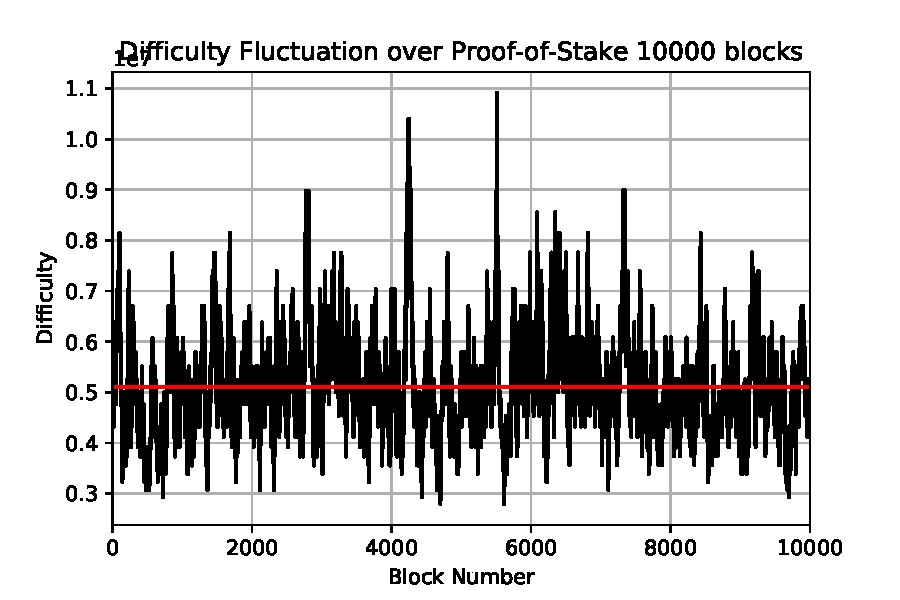
\includegraphics[width=0.55\linewidth]{assets/sim_results/pos_10000_difficulty.pdf}
    \caption{PoS difficulty over 10000 blocks. The simulation results represent
    a steady state (without perturbation of hashing or voting power). The parameters used
    were voting power = 500000, with an initial difficulty of $d_s=5000000$. Therefore we
    expect the difficulty (on average) to trend towards $d_s$, the resulting difficulty on
    average = 5109031.}
    \label{fig:pos_block_difficulty}
\end{figure}

\begin{figure}
    \centering
    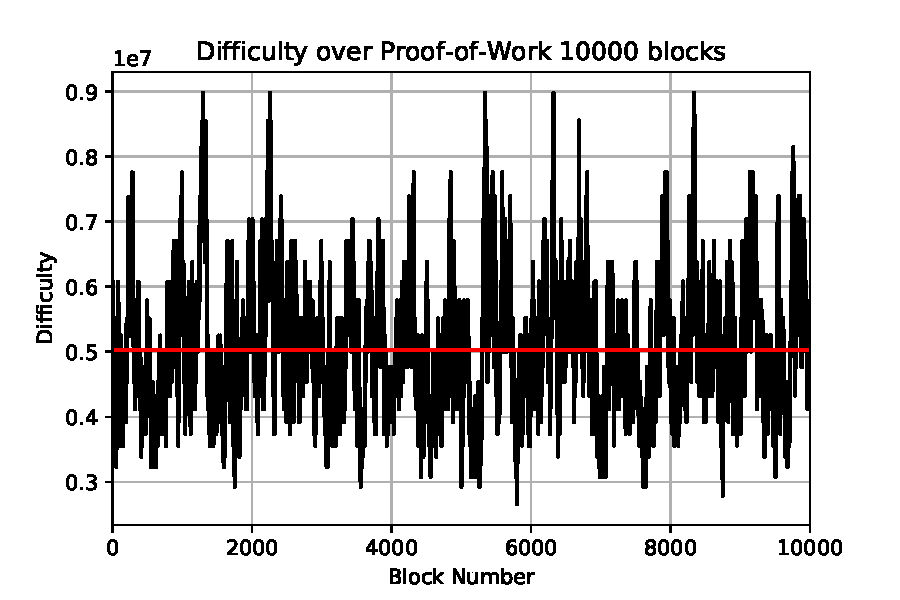
\includegraphics[width=0.55\linewidth]{assets/sim_results/pow_10000_difficulty.pdf}
    \caption{PoW difficulty over 10000 blocks, at steady state. The parameters used
    were hashing power = 500000, with an initial difficulty of $d_w=5000000$. Resulting average
    difficulty = 5027743.}
    \label{fig:pow_block_difficulty}
\end{figure}

Difficulty adjustment is tuned in the protocol to be more aggressive than the previous implementation,
that largely follows a retargeted version of the difficulty adjustment algorithm
introduced in \cite{wood2014ethereum}. Additionally, it is tuned specifically to target a
10 second block time, whereas the previous algorithm targeted a specific range. As depicted
in figures \ref{fig:pow_block_difficulty} and \ref{fig:pos_block_difficulty}, the 
adjustment algorithm can properly target the desired block time, and reaches
the expected difficulty of the network.